\documentclass[12pt]{article}

\usepackage{sbc-template}

\usepackage{graphicx,url}

\usepackage[brazil]{babel}   
%\usepackage[latin1]{inputenc}  
\usepackage[utf8]{inputenc}  
% UTF-8 encoding is recommended by ShareLaTex

     
\sloppy

\title{Exercício 6 - Laboratório de Redes de Computadores}

\author{Leonardo G. Carvalho\inst{1}, Matheus S. Redecker\inst{1}}


\address{Pontifícia Universidade Católica do Rio Grande do Sul - PUCRS
  \email{  \{leonardo.gubert\}\{matheus.redecker\} @acad.pucrs.br}
}


\begin{document} 

\maketitle

\section{}

\subitem{a) Os pacotes trocados para o handshake de estabelecimento de conexão TCP entre origem e destino foram de: \\
mensagem de TCP SYN, apresentado na figura \ref{hand1}, onde a origem faz solicitação de conexão com o destino. O destino responde com uma mensagem de TCP SYN ACK, representado na figura \ref{hand2}, onde é aceita a conexão. E por fim uma mensagem de TCP ACK, onde pode ser visto na figura \ref{hand3}, onde a origem sinaliza o destino que a conexão foi efetivamente estabelecida.
    
\begin{figure}[ht]
\centering
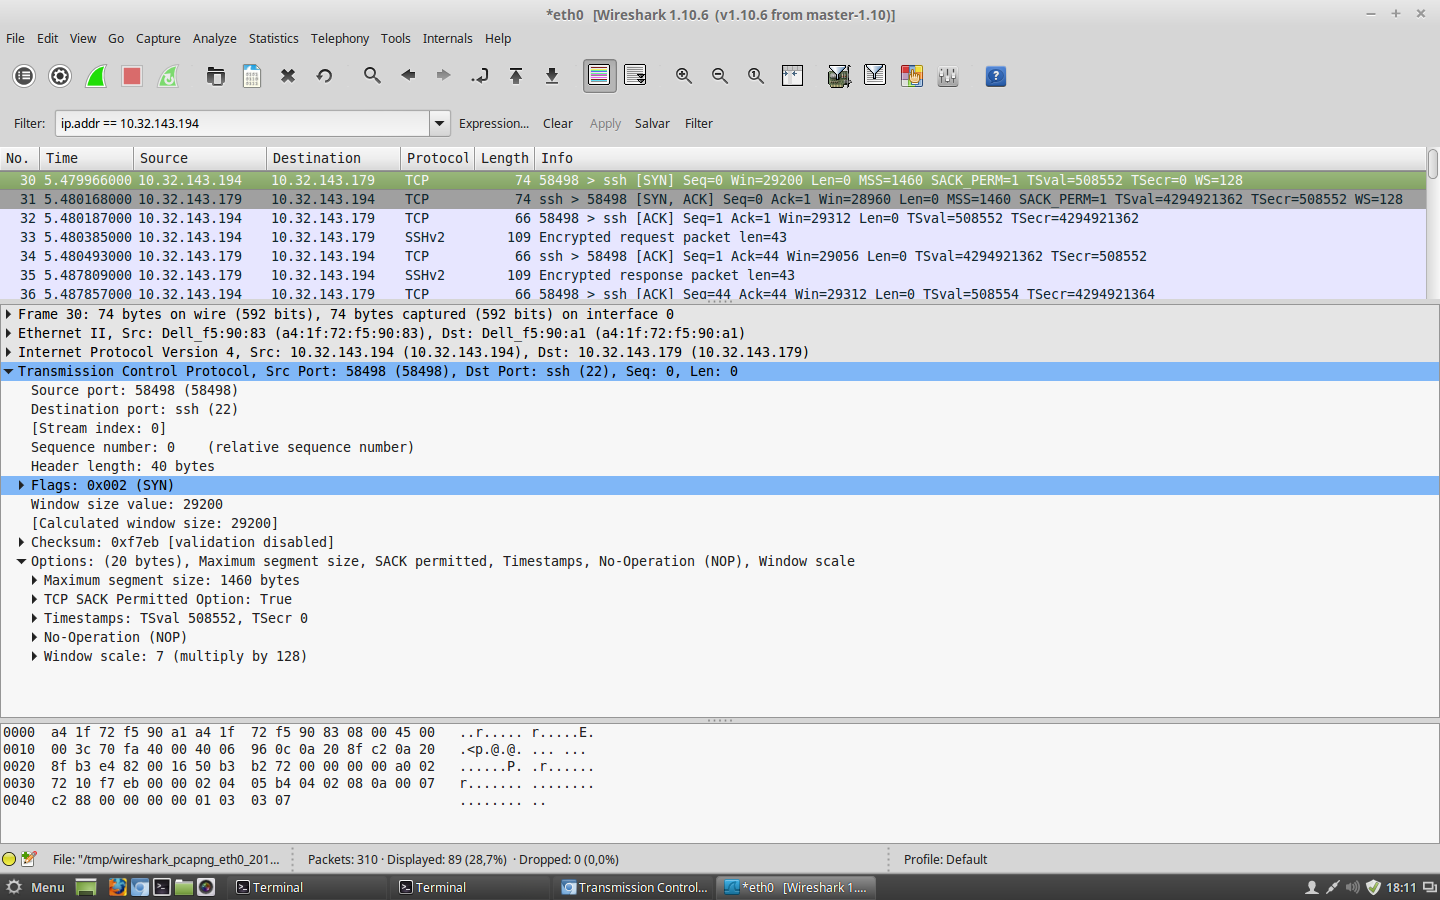
\includegraphics[scale=0.25]{handshake1.png}
\caption{}
\label{hand1}
\end{figure}


\newpage{}    
\begin{figure}[ht]
\centering
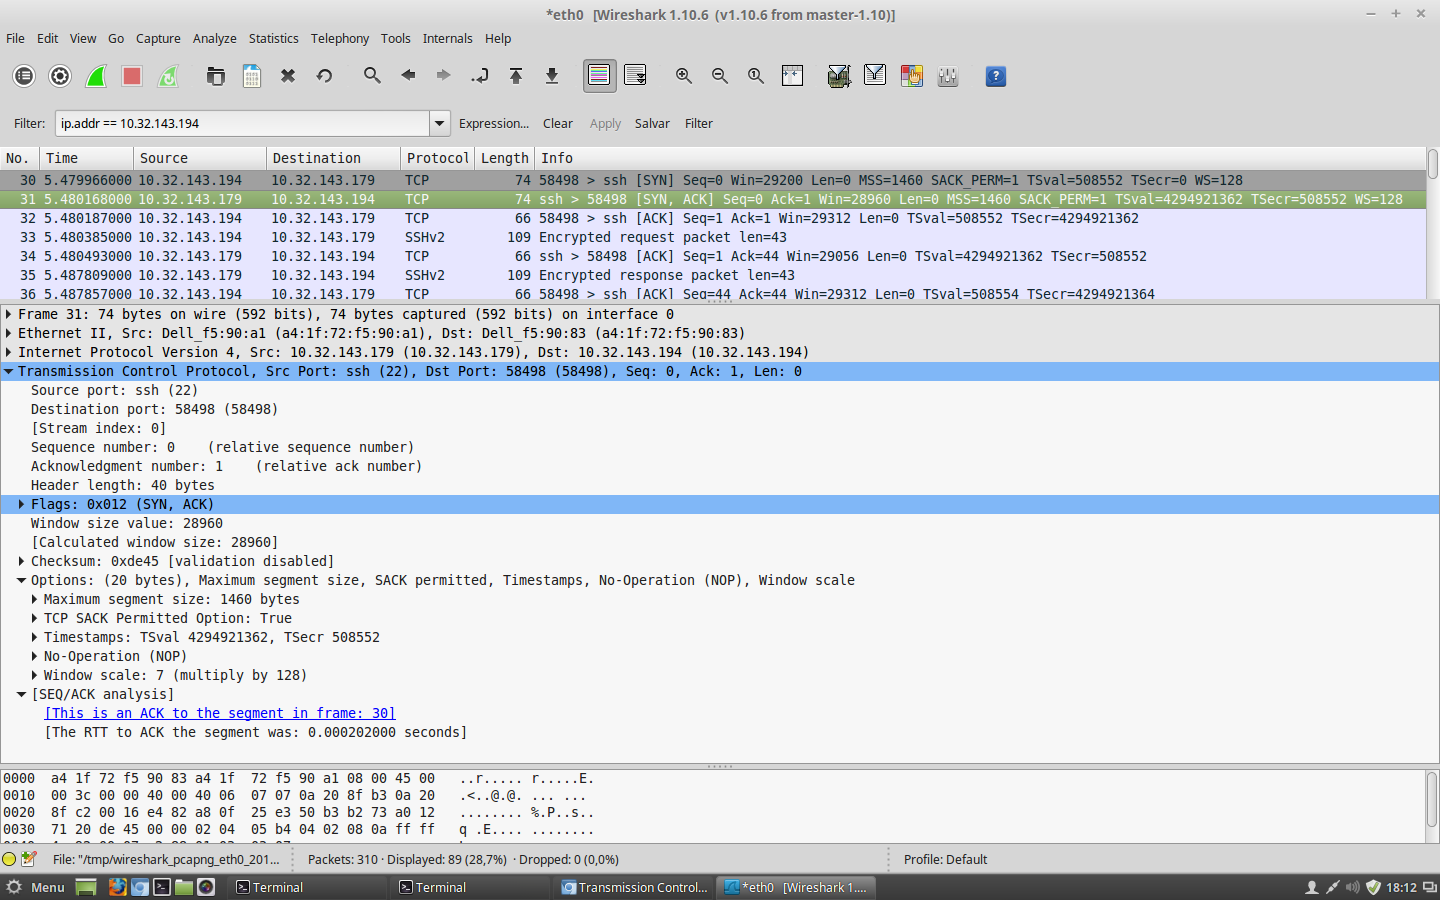
\includegraphics[scale=0.25]{handshake2.png}
\caption{}
\label{hand2}
\end{figure}

\begin{figure}[ht]
\centering
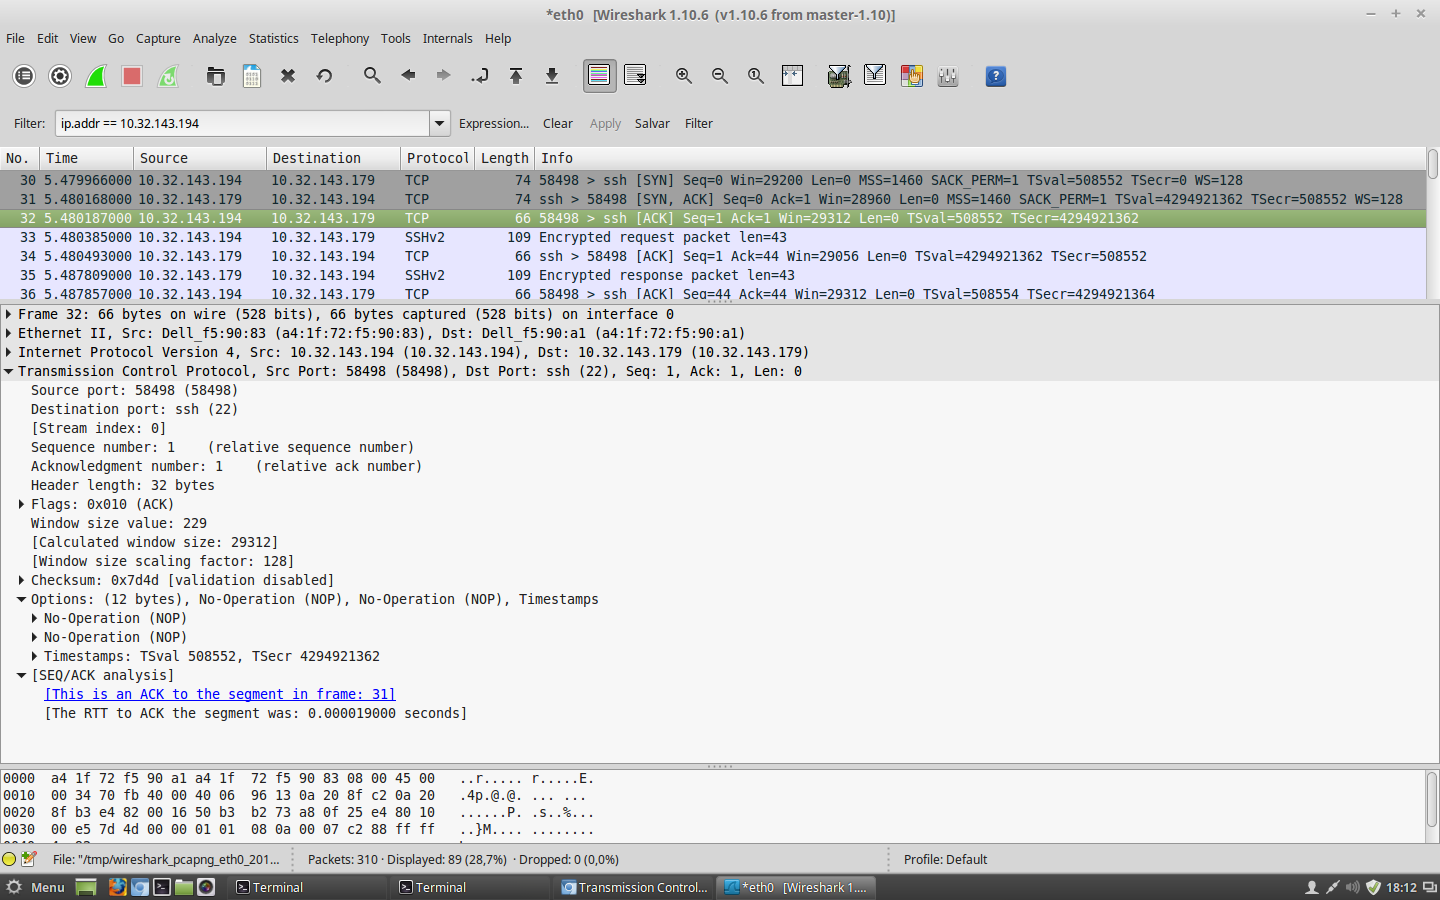
\includegraphics[scale=0.24]{handshake3.png}
\caption{}
\label{hand3}
\end{figure}

\newpage{}    
    
\subitem{b) A Origem e destino enviam seus número de seqüência iniciais para a conexão em curso. Este número deve ser alterado ao longo do tempo e ser diferente de conexão para conexão.

\section{} Para finalizar uma conexão a origem manda uma mensagem de TCP FIN ACK, apresentado na figura \ref{fimack}, onde é solicitado o fim da conexão, em seguida o destino envia uma mensagem de TCP ACK para sinalizar que está ciente que a origem deseja finalizar a conexão, como pode ser visto na figura \ref{ack}, após isso o destino envia a mensagem de TCP FIN ACK que sinaliza que a conexão foi fechada, apresentado na figura \ref{fimackdest}, e assim a origem envia a mensagem de TCP ACK para concordar com o encerramento, como pode ser visto na figura \ref{fimackori}.
\begin{figure}[ht]
\centering
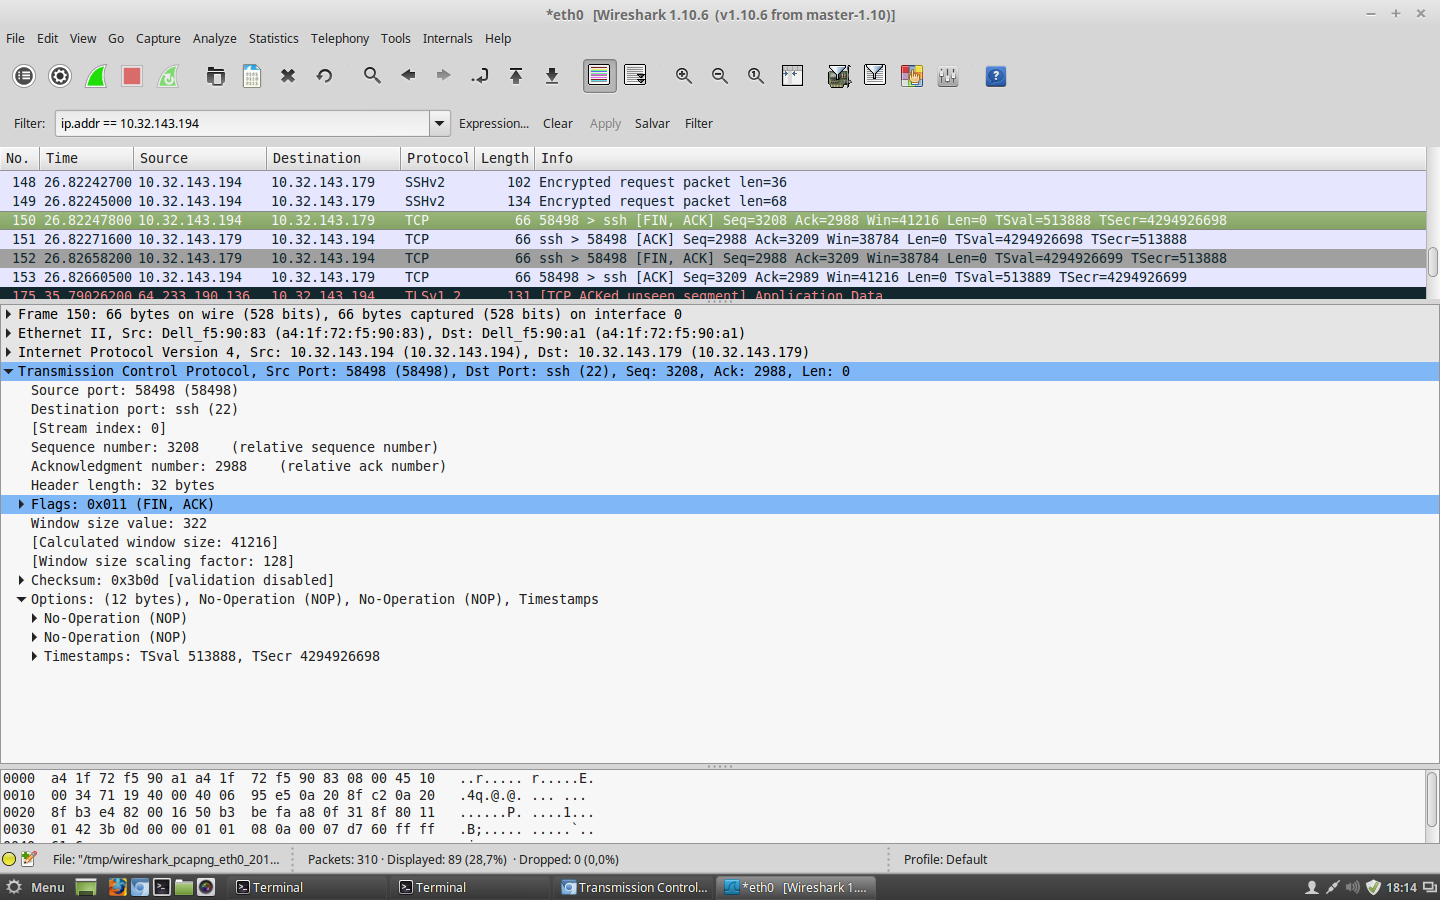
\includegraphics[scale=0.25]{fim1.png}
\caption{}
\label{fimack}
\end{figure}

\begin{figure}[ht]
\centering
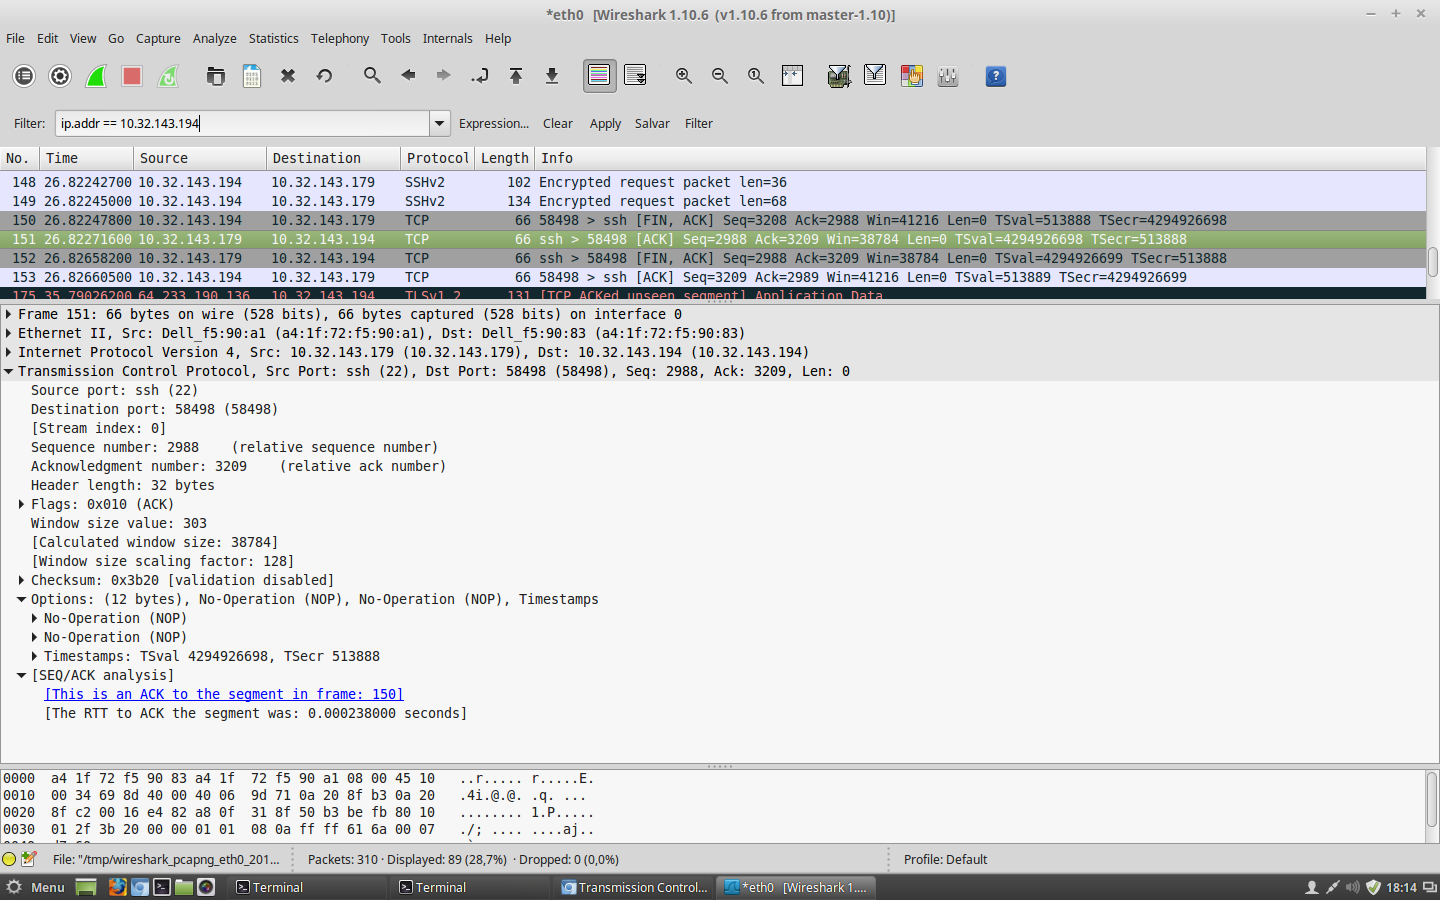
\includegraphics[scale=0.25]{fim2.png}
\caption{}
\label{ack}
\end{figure}
\newpage{}    
\begin{figure}[ht]
\centering
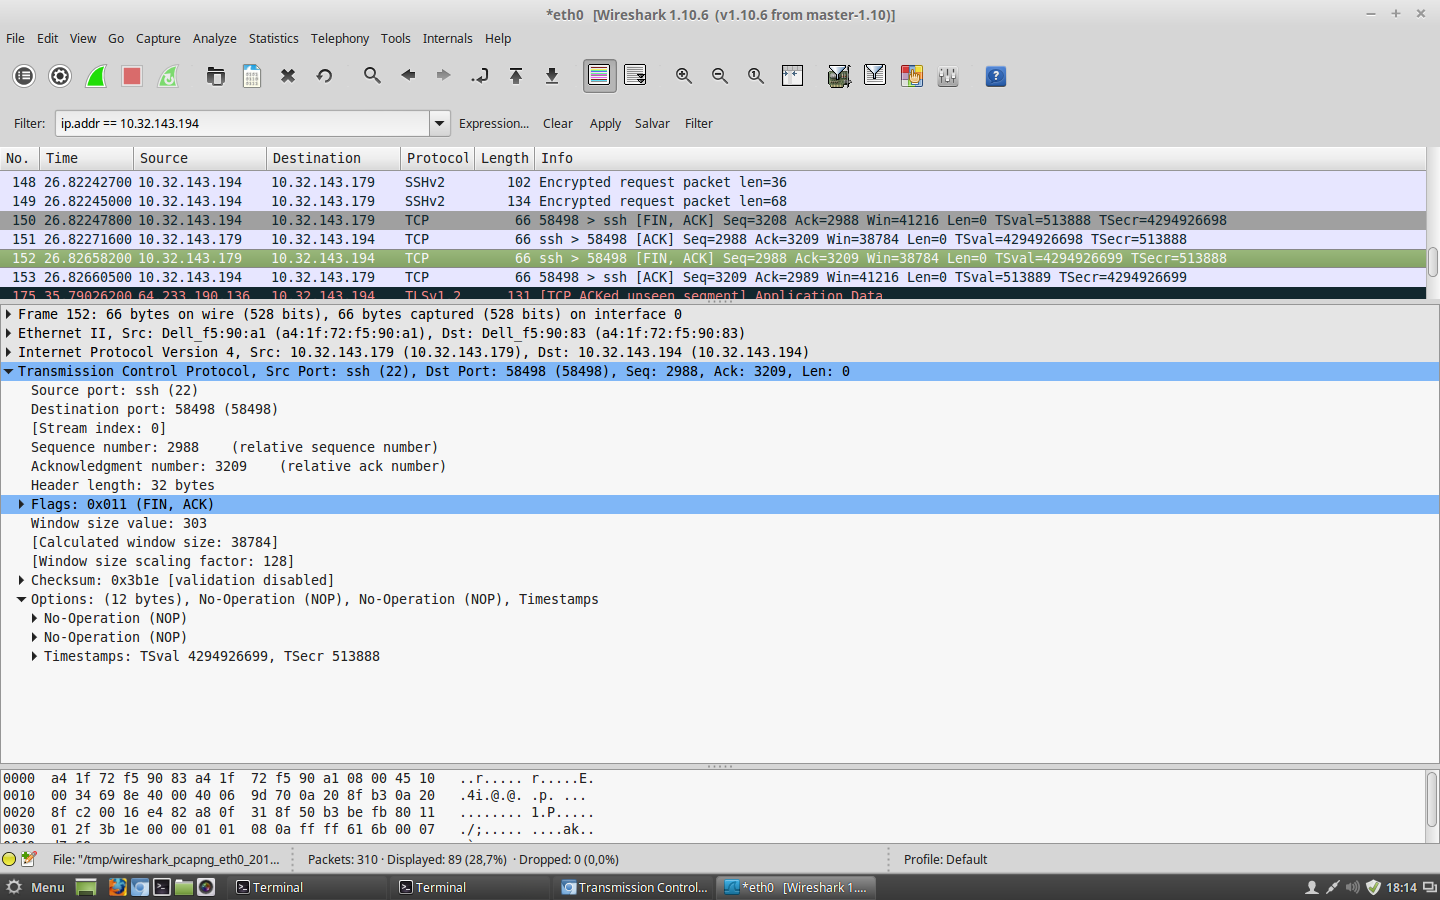
\includegraphics[scale=0.25]{fim3.png}
\caption{}
\label{fimackdest}
\end{figure}

\begin{figure}[ht]
\centering
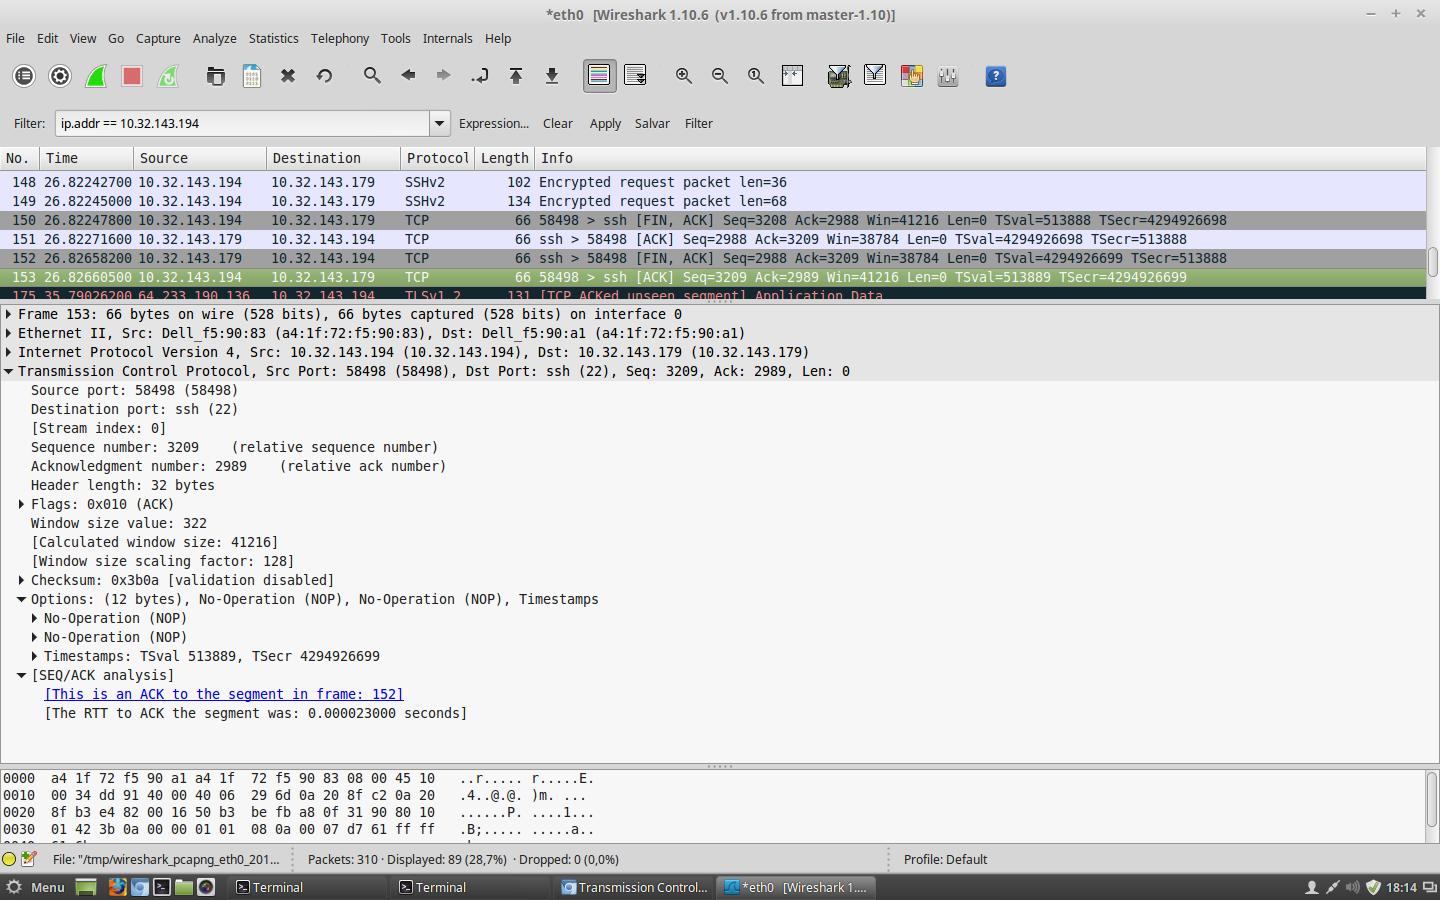
\includegraphics[scale=0.25]{fim4.png}
\caption{}
\label{fimackori}
\end{figure}
\newpage{}    
\section{}
As mensagens recebidas com a tentativa podem ser vistas nas figuras \ref{telnet1} e \ref{telnet2}.

\begin{figure}[ht]
\centering
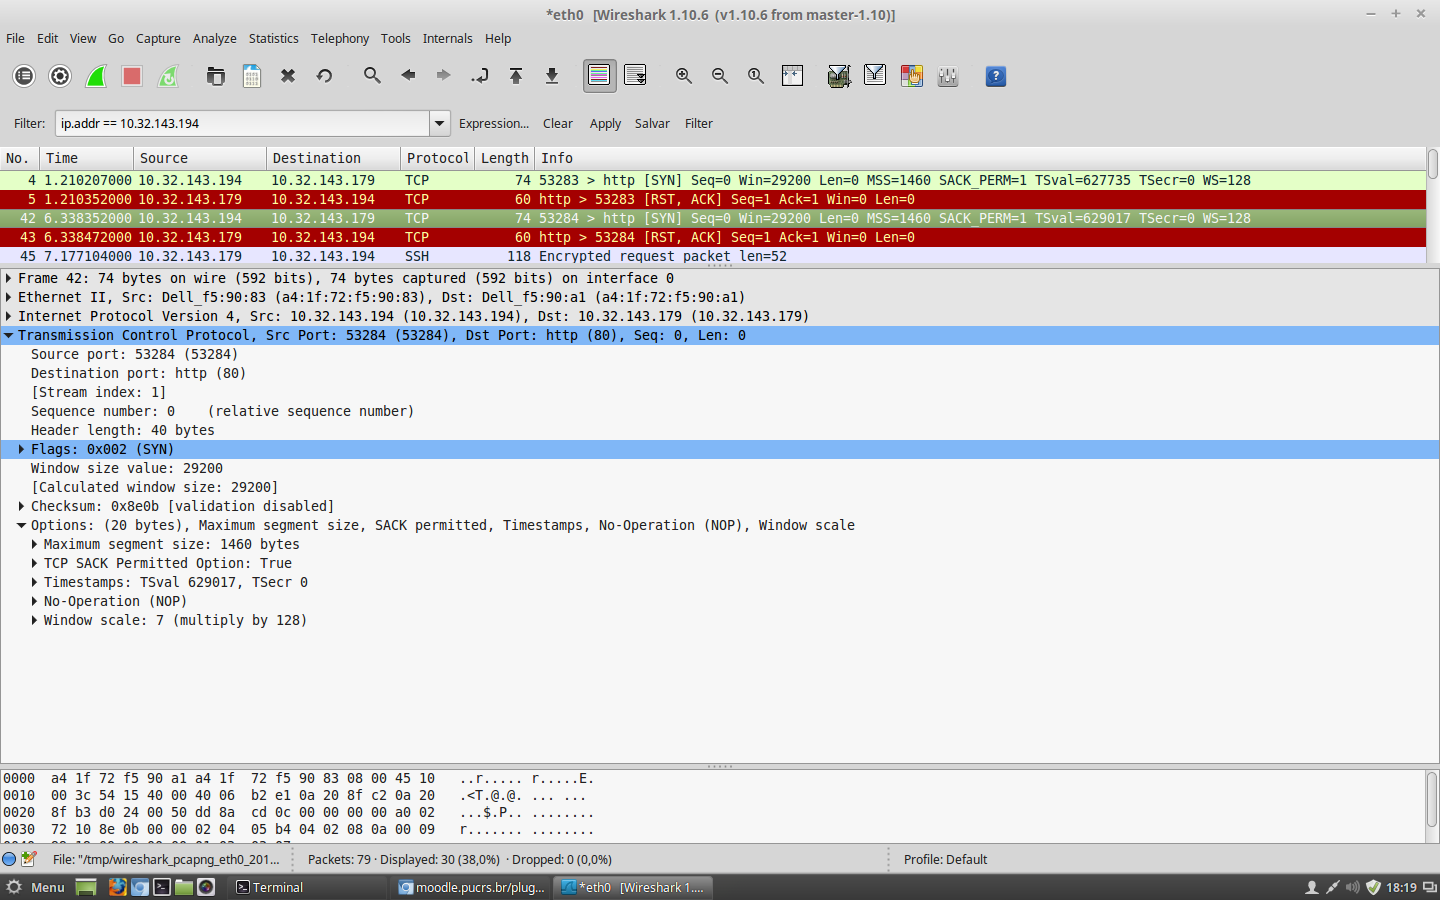
\includegraphics[scale=0.25]{telnet1.png}
\caption{}
\label{telnet1}
\end{figure}

\begin{figure}[ht]
\centering
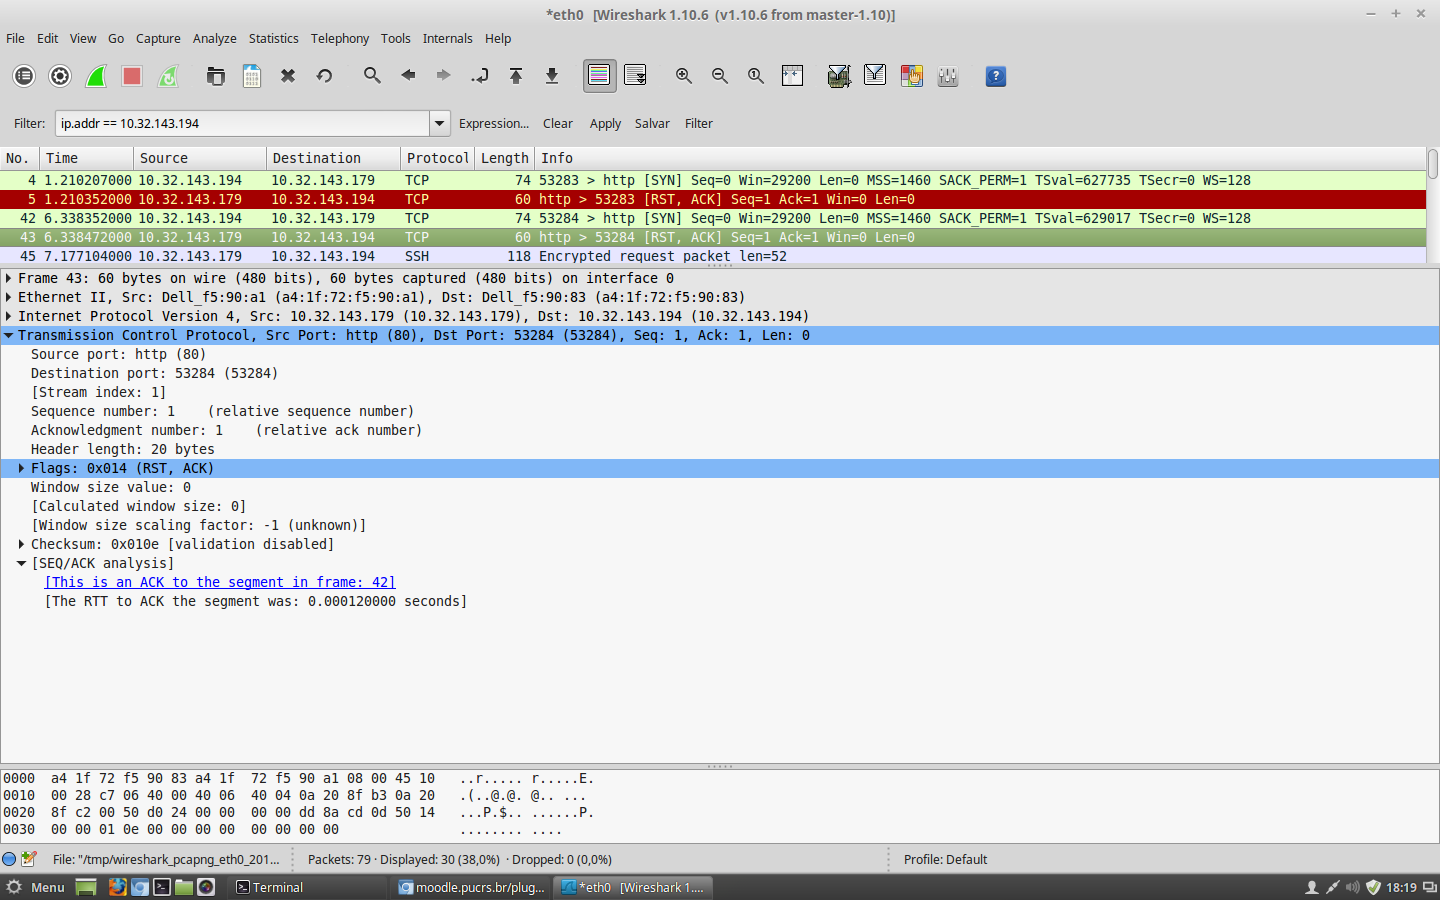
\includegraphics[scale=0.25]{telnet2.png}
\caption{}
\label{telnet2}
\end{figure}
\newpage{}    
\section{} 
Para portas que estão fechadas é recebido uma mensagem de UDP port unrecheable, que pode ser visto na figura \ref{unrech}. Já quando uma porta está aberta é concebido trafego normalmente como pode ser visto na figura \ref{certinho}.

\begin{figure}[ht]
\centering
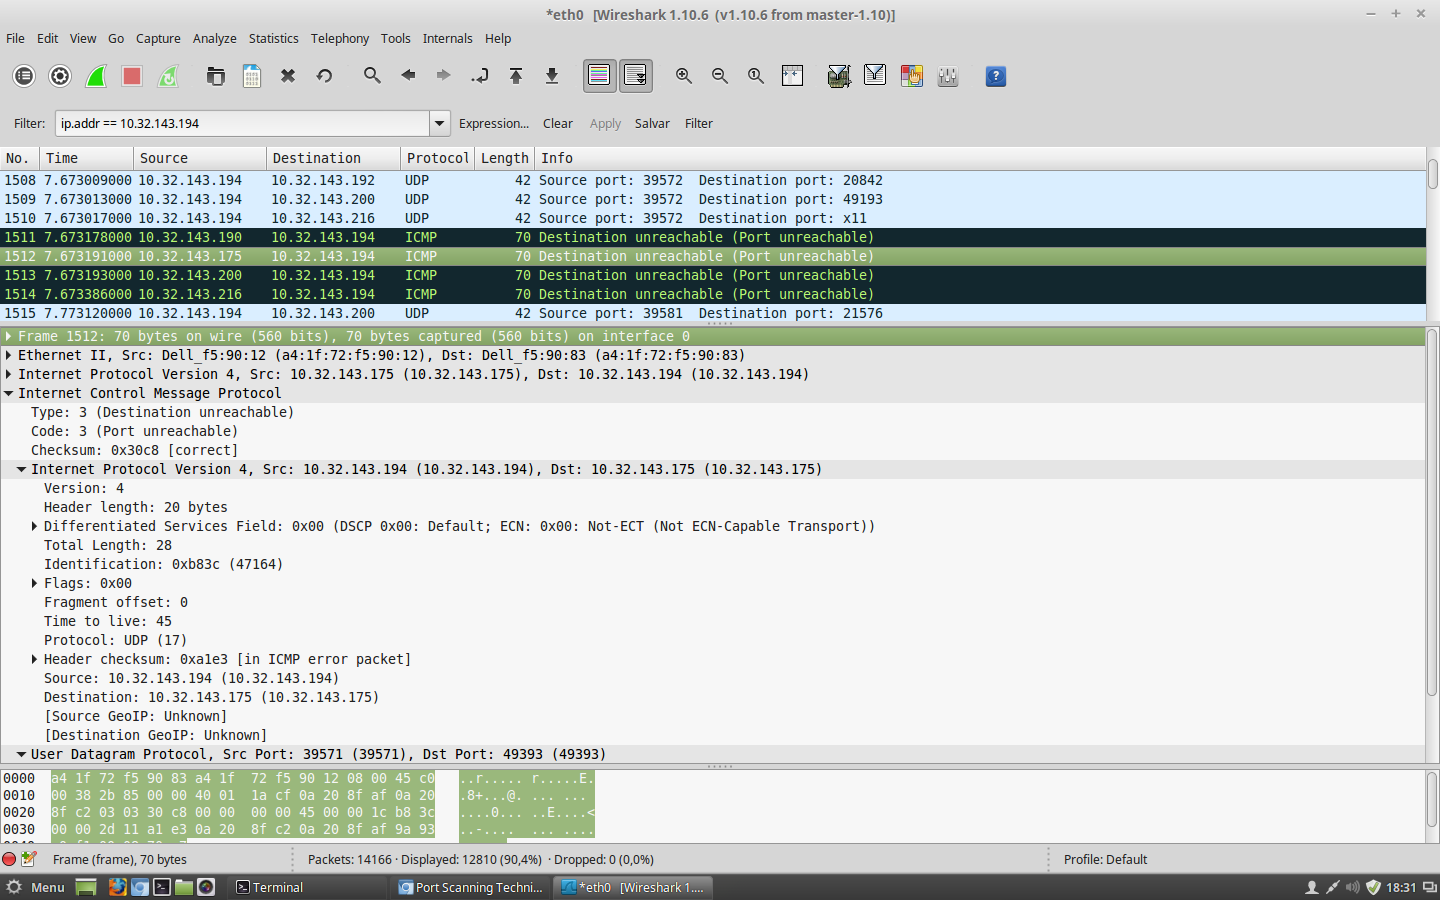
\includegraphics[scale=0.25]{udp-portUnrecheable.png}
\caption{}
\label{unrech}
\end{figure}

\begin{figure}[ht]
\centering
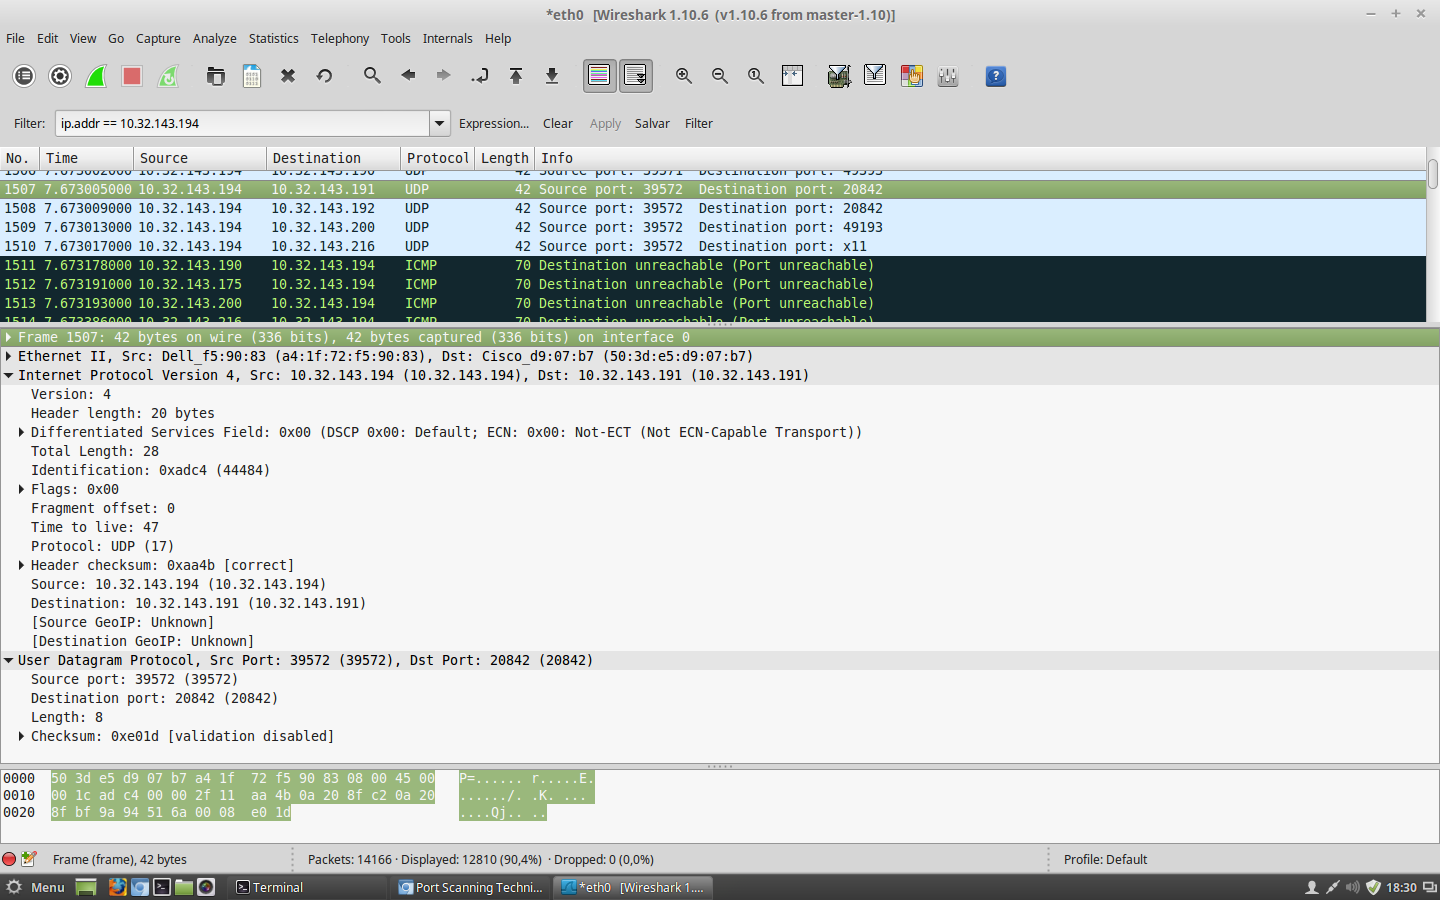
\includegraphics[scale=0.25]{udp-portaExiste.png}
\caption{}
\label{certinho}
\end{figure} 

\end{document}
